% ----------------------------------------------------------
% APÊNDICE A - Algoritmos
% ----------------------------------------------------------
\begin{apendicesenv}
\chapter{Algoritmos}
    \label{app:algoritmos}
	O algoritmo BinomialDistribution\_PROB tem como resultado a probabilidade de distribuição de um range e utiliza a fórmula  da probabilidade binomial geral abaixo. Esse algoritmo tem o mesmo resultado do algoritmo Distribution\_PROB, porém a execução do BinomialDistribution\_PROB é muito mais rápida e tem maior capacidade por usar números grandes como o BigInteger e o BigDecimal. Ambos os algoritmos foram feitos em C\# com o LINQPad 5 \footnotemark. Na Figura \ref{fig:BinomialDistribution_PROB_and_Distribution_PROB} é mostrado o resultado dos algoritmos para o range de 0 a 10, análogo ao lançamento de 10 moedas ao chão e somado os valores de caras e coras, sendo, por exemplo, a coroa com o valor um e a cara o valor dois. O algoritmo Distribution\_PROB soma cada uma das 1024 possibilidades [1,1,1,1,1,1,1,1,1,1 - 1,1,1,1,1,1,1,1,1,2 - ....] e agrupa esses valores somados. No algoritmo Distribution\_PROB esse conjunto de possibilidades é um produto cartesiano das possíveis combinações, o que torna esse algoritmo lento rapidamente, porém ele é importante para validar e facilitar o entendimento da a fórmula da probabilidade binomial geral utilizada no algoritmo BinomialDistribution\_PROB \cite{mathisfun_binomial_distribution}. Na Figura \ref{fig:BinomialDistribution_PROB_and_Distribution_PROB}, a tabela no interior de  Distribution\_PROB mostra esse agrupamento e o total de possibilidades, 1024. Ao dividir cada valor agrupado pelo total tem-se o resultado probabilístico alcançado pela fórmula empregada no BinomialDistribution\_PROB. Por exemplo, a probabilidade do somatório das 10 moedas lançadas ser 12 é igual a 45/1024, que é 0,0439453125 ou 4,39\%.
\footnotetext{O LINQPad 5 é encontrado em \url{www.linqpad.net} e pode ser utilizado em sua versão livre, Standard edition, sem expiração.}
\begin{align*}
f(k;n,p) &= \binom{n}{k} p^k(1 - p)^{n-k}
\end{align*}

\begin{figure}[H]
\caption{Resultado dos algoritmos  BinomialDistribution\_PROB e Distribution\_PROB}
\label{fig:BinomialDistribution_PROB_and_Distribution_PROB}
\centering
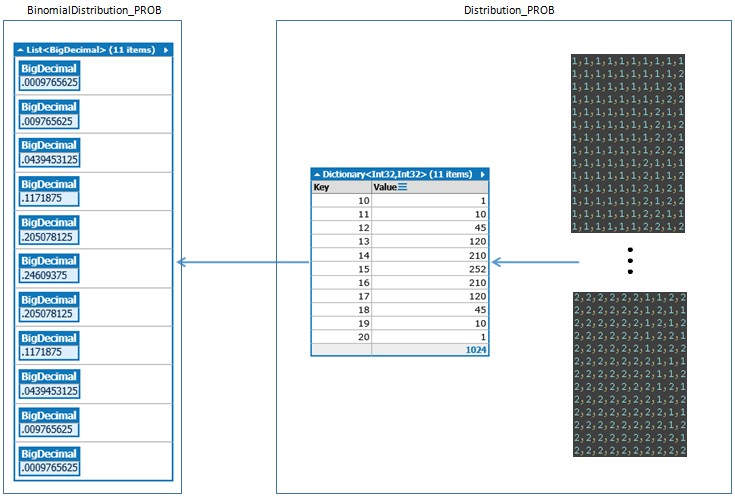
\includegraphics[scale=.75]{sections/images/BinomialDistribution_PROB_and_Distribution_PROB.jpg}
\floatfoot{O algoritmo Distribution\_PROB tem o intuito que clarificar a essência probabilística do teorema central do limite.} %\footnotemark.
\end{figure}

O algoritmo Distribution\_PROB também pode ser utilizado para o lançamento de 5 dados de 6 lados ou 6 dados de 5 lados, por exemplo. Como pode ser observado na Figura abaixo, a distribuição das probabilidades no lance dos dados é semelhante à distribuição binomial, das moedas.

\begin{figure}[H]
\centering
	\begin{subfigure}[H]{0.47\linewidth}
	\centering
	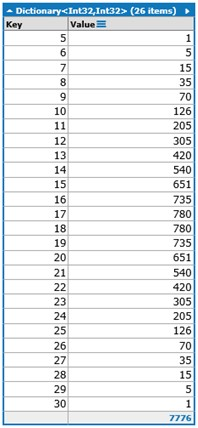
\includegraphics[width=.7\linewidth]{sections/images/Distribution_PROB_5_6.jpg}
	\caption{5 dados de 6 lados}
	\label{fig:Distribution_PROB_5_6}
	\end{subfigure}
\hfill
	\begin{subfigure}[H]{0.47\linewidth}
	\centering
	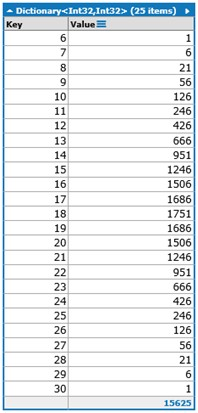
\includegraphics[width=.72\linewidth]{sections/images/Distribution_PROB_6_5.jpg}
	\caption{6 dados de 5 lados}
	\label{fig:Distribution_PROB_6_5}
	\end{subfigure}%
\caption{Resultados do algoritmo Distribution\_PROB}

\floatfoot{A distribuição das probabilidades no lance dos dados é consonante à distribuição binomial.} %\protect\footnotemark
\end{figure}

\subsection*{BinomialDistribution\_PROB}
Para execução deste trecho de código é necessário a implementação do BigDecimal, um exemplo dessa implementação, pode ser observado, obedecendo os direitos de licença de software proprietários em \cite{ github_bigdecimal}. Este estudo não distribui e nem se responsabiliza pela porção do código referente à implementação do BigDecimal, ficando essas responsabilidades  à cargo do executor deste trecho de software.

\bigbreak
\begin{lstlisting}
//https://www.mathsisfun.com/data/quincunx-explained.html
void Main()
{
    BinomailDistribuition.Possibilities = 10;
    var results = new List<BigDecimal>();
    results.Load();
    results.Print(true); //send false to print Table 1.
}

public static class BinomailDistribuition
{
    public static int Possibilities = 0;
    static int middleLeft = 0;
    static int middleRight = 0;
    static int resultCount = 0;
    
    public static void Load(this List<BigDecimal> results)
    {
        for (int i = 0; i <= Possibilities; i++)
        {
            var fatorLeft = Fatorial(Possibilities);
            var fatorRight = BigInteger.Multiply(Fatorial(i), Fatorial(Possibilities - i));
            BigInteger fat = BigInteger.Divide(fatorLeft, fatorRight);
            var powLeft = new BigDecimal(1, 0, 1000000000);
            var powRight = new BigDecimal(1, 0, 1000000000);
            if (i != 0)
                powLeft = BigDecimal.Pow(new BigDecimal(5, 1, 1000000000), i);
            if (i != Possibilities)
                powRight = BigDecimal.Pow(new BigDecimal(5, 1, 1000000000), (Possibilities - i));
            var prob = new BigDecimal(fat) * powLeft * powRight;
            results.Add(prob);
        }
    }
    
    public static BigInteger Fatorial(int value)
    {
        BigInteger fatorial = 1;
        for (int n = 1; n <= value; n++)
        {
            fatorial *= n;
        }
        return fatorial;
    }
    
    public static void Print(this List<BigDecimal> results, bool printTableProbability)
    {
        if (!printTableProbability)
        {
            var sum = results.Sum();
            var middle = (middleRight - middleLeft) / 2;
            var middlePercent = ((middleRight - middleLeft) * 14) / 100;
            var list = results.Where((x, i) => i >= middleLeft && i <= middleRight).ToList();
            var listPareto = list.Where((x, i) => i >= (middle - middlePercent) && i <= (middle + middlePercent)).ToList();
            var percentOfSum = (middleRight - middleLeft) * 100 / resultCount;
            var sumPercent = sum * new BigDecimal(100, 0, 1000000000);
            var paretoResult = new BigDecimal(0, 0, 1000000000);
            listPareto.ForEach(x => { paretoResult = paretoResult + x; });

            sumPercent.Dump("sum");
            middleLeft.Dump("middleLeft");
            middleRight.Dump("middleRight");
            (middleRight - middleLeft).Dump("itens of sum");
            percentOfSum.Dump("percent of sum");
            resultCount.Dump("total");
            paretoResult.Dump("20/80");
        }
        else
        {
            results.Dump(); //Valid Binomial distribution    
        }
    }
    
    public static BigDecimal Sum(this List<BigDecimal> results)
    {
        resultCount = results.Count;
        middleLeft = resultCount / 2;
        middleRight = middleLeft * 2 < resultCount ? middleLeft + 1 : middleLeft;

        var sum = middleLeft != middleRight ? results[middleLeft] + results[middleRight] : results[middleRight];
        while ((sum * new BigDecimal(100, 0, 1000000000)) < new BigDecimal(9999, 2, 1000000000))
        {
            middleLeft--;
            middleRight++;
            if (middleLeft >= 0)
                sum = sum + results[middleLeft];
            if (middleRight <= Possibilities)
                sum = sum + results[middleRight];
        }
        return sum;
    }
}

//Exemple of BigDecimal class - https://github.com/dparker1/BigDecimal/blob/
//3e0a4f1ba4c72c0b28d6571fcc6259558be104bd/BigDecimal/BigDecimal.cs
\end{lstlisting}

\bigbreak
\bigbreak
\subsection*{Distribution\_PROB}
\begin{lstlisting}
//https://exercicios.brasilescola.uol.com.br/exercicios-matematica/
//exercicios-sobre-probabilidade-condicional.htm#questao-1
void Main()
{
    var dice = 2; //Binomial distribution, dice = 2;
    var events = 10;
    var sampling = Math.Pow(dice, events);
    var cartesianProduct = dice.ToArrays(events).CartesianProduct();
    cartesianProduct.PrintGroup(events, dice);
}

public static class CartesianProductContainer
{
    public static IEnumerable<IEnumerable<int>> CartesianProduct(this IEnumerable<IEnumerable<int>> sequences)
    {
        IEnumerable<IEnumerable<int>> emptyProduct = new[] { Enumerable.Empty<int>() };
        var result = sequences.Aggregate(
            emptyProduct,
            (accumulator, sequence) =>
                from accseq in accumulator
                from item in sequence
                select new[] { accseq.Concat(new[] { item }).Sum() });

        return result;
    }

    public static IEnumerable<List<int>> ToArrays(this int dice, int events)
    {
        var result = new List<List<int>>();
        for (int j = 1; j <= events; j++)
        {
            var array = new List<int>();
            for (int i = 1; i <= dice; i++)
                array.Add(i);
            
            result.Add(array);
        }

        return result;
    }
    
    public static void PrintGroup(this IEnumerable<IEnumerable<int>> list, int events, int dice)
    {
        var listCountDict = Enumerable.Range(1, dice * events).ToDictionary(x => x);
        Group(listCountDict, list);
        listCountDict.Dump("Values");
    }

    public static void Group(Dictionary<int, int> dict, IEnumerable<IEnumerable<int>> list)
    {
        foreach (var key in dict.Keys.ToList())
            dict[key] = 0;

        foreach (var item in list)
            dict[item.First()]++;

        var zeroKey = 0;
        foreach (var item in dict)
            if (item.Value == 0) 
                zeroKey = item.Key;
            else continue;

        for (int i = 1; i <= zeroKey; i++)
            dict.Remove(i);
    }
}

\end{lstlisting}


\end{apendicesenv}